
\newcommand{\hgline}[2]{
\pgfmathsetmacro{\thetaone}{#1}
\pgfmathsetmacro{\thetatwo}{#2}
\pgfmathsetmacro{\theta}{(\thetaone+\thetatwo)/2}
\pgfmathsetmacro{\phi}{abs(\thetaone-\thetatwo)/2}
\pgfmathsetmacro{\close}{less(abs(\phi-90),0.0001)}
\ifdim \close pt = 1pt
    \draw[black!70] (\theta+180:1) -- (\theta:1);
\else
    \pgfmathsetmacro{\R}{tan(\phi)}
    \pgfmathsetmacro{\distance}{sqrt(1+\R^2)}
    \draw[black!70] (\theta:\distance) circle (\R);
\fi
}
\begin{figure}
    \centering
    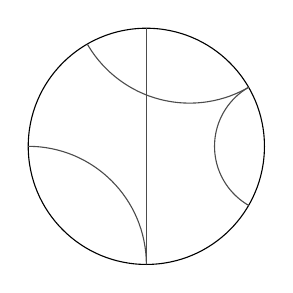
\begin{tikzpicture}[scale=1.5]
        \draw (0,0) circle (1);
        \clip (0,0) circle (1);
        \hgline{30}{-30}
        \hgline{180}{270}
        \hgline{30}{120}
        \hgline{0}{180}
        
    \end{tikzpicture}
    \label{fig:hyperbolicGeodesics}
    \caption{Geodesics in the Poincaré ball model.}

\end{figure}